\documentclass[../main.tex]{subfiles}

\begin{document}
\subsection{Implementation Plan}
TrackMe system is composed of five macro components (\textit{fig. 2}) that can be developed independently and simultanously
after interfaces and communications standards are properly chosen.\\



\subsection{Integration Plan}
Although macro components will be developed indipendently, it is strongly suggested a top-down approach oriented towards functionalities
implementation. 
 \subsubsection{Mobile Client, Applications and Database Servers}
    The first thing to be developed will be the "core functionality of the system" and Data4Help (\textit{Fig. 17}). Then it will be possible
    to test the backbone of the system (servers communication, models and APIs). Following the same approach, the development will focus consequently on
    AutomatedSOS and then on Track4Run.

    
 \subsubsection{Web Server}
    Being a totally independent part of the system, the Web Server will be developed by a different team or after the development of the other components.\\
    The APIs documentation to be hosted on the Web Server will be produced by the Data4Help Application server developers. 
\subsection{Test Plan}
    Following the top-down approach, each module should be tested as soon as it is completed and integrated progressively.\\
    Single modules development will implement Continous Integration practices to speed up development.
    It is advised to implement a \textit{Gated Commit} pattern to avoid "code breaking" commits to the master codebase, that ultimatly will delay
    TrackMe development 
    \begin{figure}[H]
        \centering
             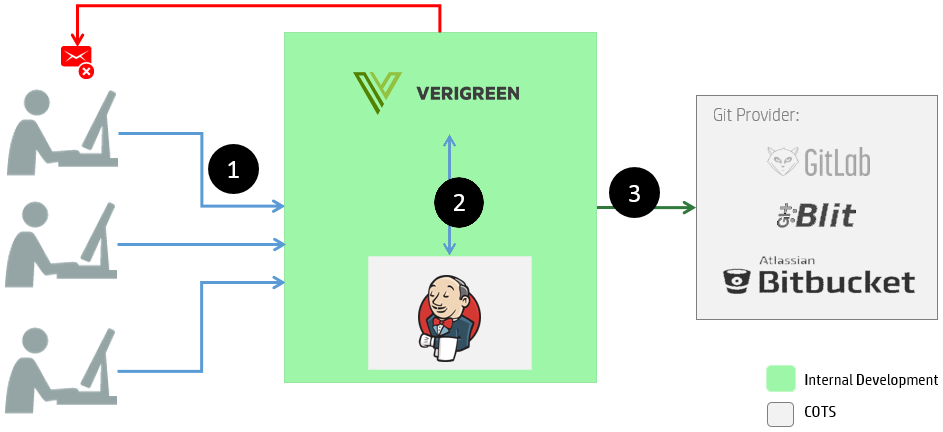
\includegraphics[width=1.0\textwidth]{gated_commit.png}
              \caption{A gated commit pattern using a \textit{jenkins} server with \textit{Verigreen}}
               \label{fig:gated_commit}
    \end{figure}
\subsubsection{System Testing}
    The application will be firstly beta tested in the urban area of Milan, thus it will be possible
    to gather statistics about application usage and user base to better plan a final release.\\
    The system must be able to withstand constant data upload from our users, it's advised a load test.\\
    We expect companies to make a large volume of request to Data4Help server, so it should be subject to load and stress tests.
\subsection{API testing}

    It's critical to test the correct behaviour of TrackMe API. The best approach will be to use a dedicated software like \textit{POSTMAN} to test API as soon as they are developed.
    \begin{figure}[ht]
        \centering
             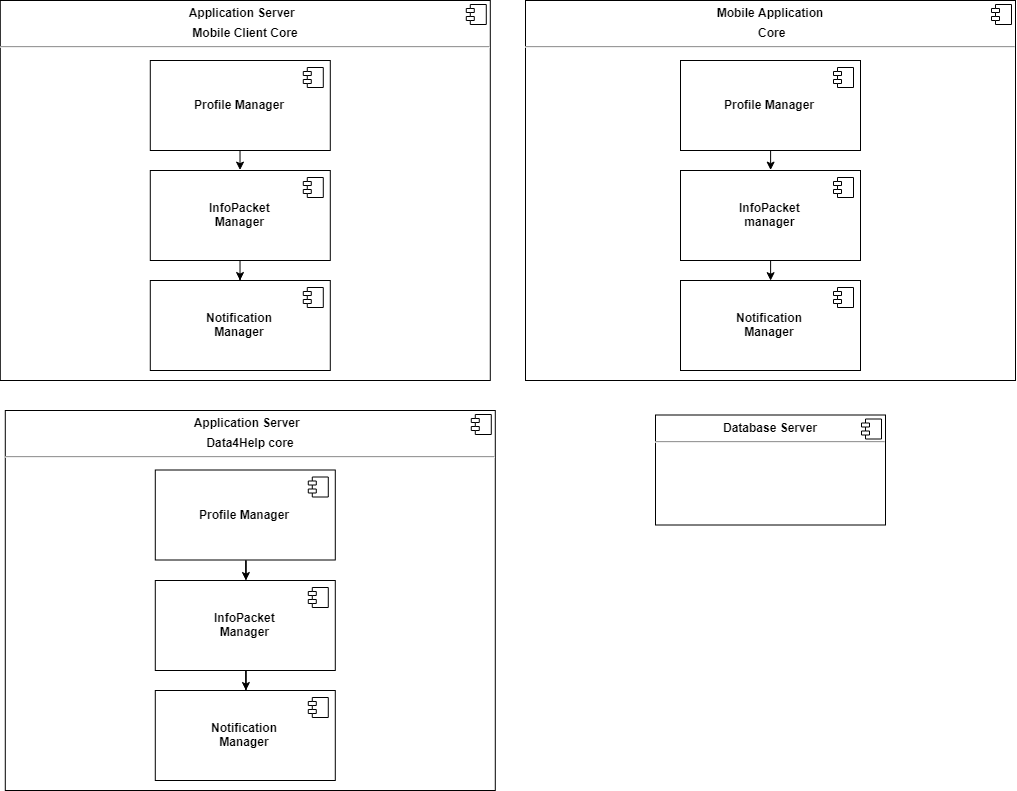
\includegraphics[width=1.0\textwidth]{development.png}
              \caption{core functionality development}
               \label{fig:development}
    \end{figure}
 
\end{document}
